\newpage

\section*{ANEXOS}

\subsection*{ANEXO A - ÁRBOL DE PROBLEMAS}
\vspace{30mm}
\begin{center}
    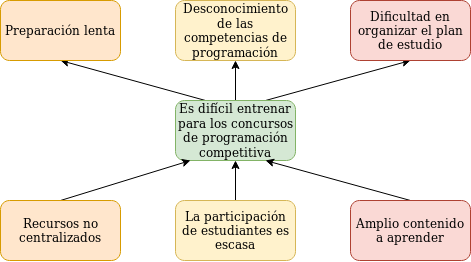
\includegraphics[scale=0.9]{imagenes/arbol de problemas.png}
\end{center}

\newpage
\subsection*{ANEXO B - ÁRBOL DE OBJETIVOS}
\vspace{30mm}
\begin{center}
    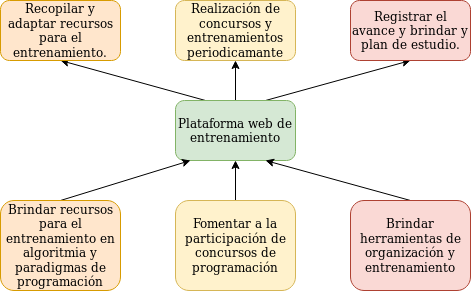
\includegraphics[scale=0.9]{imagenes/arbol de objetivos.png}
\end{center}

\newpage
\subsection*{ANEXO C - MARCO LÓGICO}
\begin{center}
    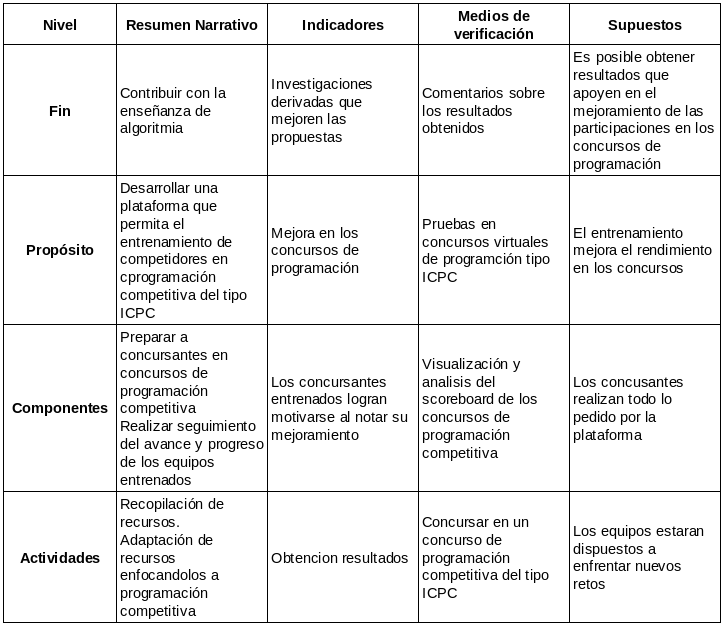
\includegraphics[scale=1.2]{imagenes/marco logico.png}
\end{center}
% \footnotesize
% {\setstretch{1.0}
% \begin{center}
%     \begin{tabularx}{\textwidth}{|l|X|X|X|X|}
%         \hline
%         Nivel &	Resumen narrativo &	Indicadores & Medios de verificacion & Supuestos\\
%         \hline
%         Fin & Contribuir con el desarrollo de la conducción autónoma & Investigaciones derivadas que mejores las propuestas &	Tesis derivadas y comentarios sobre los resultados obtenidos &	Es posible obtener resultados que apoyen en el avance de la conducción autónoma\\
%         \hline
%         Propósito & Desarrollar un flujo que permita el entrenamiento de modelos de aprendizaje profundo que combinados con algoritmos de visión computacional logren una conducción autónoma básica en pistas y carreterasDesarrollar un flujo que permita el entrenamiento de modelos de aprendizaje profundo que combinados con algoritmos de visión computacional logren una conducción autónoma básica en pistas y carreteras & Rendimiento de la los algoritmos y modelos & Pruebas en un simulador & Los algoritmos y modelos dan buenas predicciones\\
%         \hline
%         Componentes & 
%         \begin{itemize}[nosep]
%             \item Diseñar un componente de aumentación y preprocesamiento de datos para extraer la información útil de los datasets y fuentes de datos disponibles.
%             \item Reducir la complejidad de la implementación del flujo mediante el uso de sólamente cámaras.
%             \item Implementar un componente que combine la predicción algoritmos de visión computacional y modelos de aprendizaje profundo para mejorar la generalización de predicciones.
%             \item Analizar y entrenar modelos de aprendizaje profundo con una alta exactitud en las predicciones utilizando menos requisitos de cómputo.
%             \item Evaluar las predicciones de los modelos entrenados para comprobar si las representaciones aprendidas son invariantes a los cambios de perspectiva e iluminación.
%         \end{itemize} & 
%         \begin{itemize}[nosep]
%             \item los datos son útiles para el entrenamiento
%             \item disminución de la complejidad
%             \item generalización en distintas situaciones de entrada
%             \item \% de exactitud en las predicciones
%             \item invarianza en perspectiva e iluminación
%         \end{itemize} & 
%         "Métricas del error para medir el rendimiento de los modelos
% Visualización de las representaciones aprendidas" &
%         \begin{itemize}[nosep]
%             \item datos con información importante para la tarea
%             \item es posible realizar la tarea sólo con cámaras
%             \item algoritmos de visión computacional funcionan bien junto con modelos de aprendizaje profundo
%             \item es posible lograr una alta exactitud en la predicción
%             \item es posible aprender representaciones invariantes
%         \end{itemize}\\
%         \hline
%     \end{tabularx}\\
% \end{center}
% }